\documentclass[/home/hernan/Documentos/Apuntes_mecanica_teorica/main.tex]{subfiles}
\graphicspath{{\subfix{images/}}}

\begin{document}
	\part{Mecánica Newtoniana} 
	\label{prt:Mecánica Newtoniana}

	\section{Vectores}\label{sec:vectores}


	Esto ya deberían saberlo y probablemente se actualice de último $: \left . \right)$

	\newpage
	\section{Mecánica Newtoniana para una partícula}\label{sec: N.particula }

	A continuación se expresará la mecánica de partículas.

	\subsection{Leyes de Newton}
	
	Comenzando con algunos conceptos claves para el desarrollo de las leyes de Newton:

	\begin{definition}[\textbf{Fuerza}]
		Fuerza es el nombre que se le da a la interacción entre un cuerpo y su entorno, la cual es capaz de afectar el estado del cuerpo. Las fuerzas son cantidades vectoriales, por lo que poseen magnitud y dirección; su magnitud es dada en unidades de newton $N$.
	\end{definition}

	\begin{definition}[\textbf{Momentum Lineal}]
		Momentum lineal o cantidad de movimiento, ambos se refieren a una cantidad vectorial dada por la siguiente ecuación:
		\begin{equation}
			\vec{p} = m \vec{v}
			\label{eq: momentuml}
		\end{equation}
	\end{definition}

	\marginnote{Un estado de \textbf{equilibrio} se refiere a que el cuerpo o sistema de interés se encuentra movientodose con velocidad lineal constante (\textbf{equilibrio dinámico}) o se encuentra en reposo (\textbf{equilibrio estático}). \vspace{2cm}}
	
	Las leyes de Newton tal y como se expresarán a continuación son unicamente válidas para sistemas de referencias \textbf{inerciales}, es decir, sistemas de referencia que no poseen ningun tipo de aceleración.


	\begin{definition}[\textbf{Primera Ley de Newton o  Ley de la Inercia}]
		Un cuerpo mantiene su estado de equilibrio a menos de que una fuerza neta diferente de cero lo perturbe. Dicho de otra forma, un cuerpo siempre mantendrá su estado de equilibrio a menos de que una fuerza neta llegue a afectarlo.
		\begin{equation}
			\sum \vec{F} = \vec{0}
			\label{eq: Nfirstlaw}
		\end{equation}
		
	\end{definition}

	
	\begin{definition}[\textbf{Segunda Ley de Newton}]
		Un cuerpo que experimenta una fuerza neta diferente de cero, tendrá como resultado un cambio en su momentum lineal.
		
		\begin{equation}
			\sum \vec{F} = \frac{d \vec{p}}{dt} = \dot{\vec{p}}
			\label{eq: NSecondlaw}
		\end{equation}

		Suponiendo que la masa es constante para el cuerpo de interés, la primera ley de Newton también se puede escribir de la forma:

		\begin{equation}
			\sum \vec{F} = m \vec{a}
		\end{equation}
	\end{definition}


	\begin{marginfigure}
		\begin{figure}[H]
			\centering
			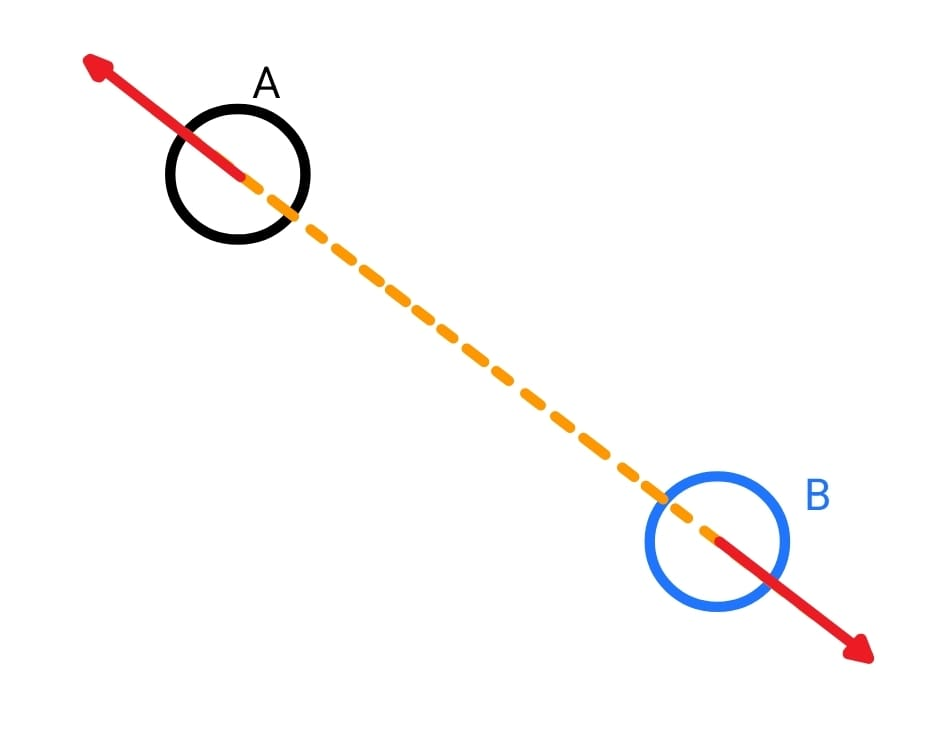
\includegraphics[width=4.5cm]{strongthirdlaw.jpeg}
			\caption{Situación del enunciado fuerte}
			\label{fig: Nthirdstrong}
		\end{figure}
	\end{marginfigure}

	\begin{marginfigure}
		\begin{figure}[H]
			\centering
			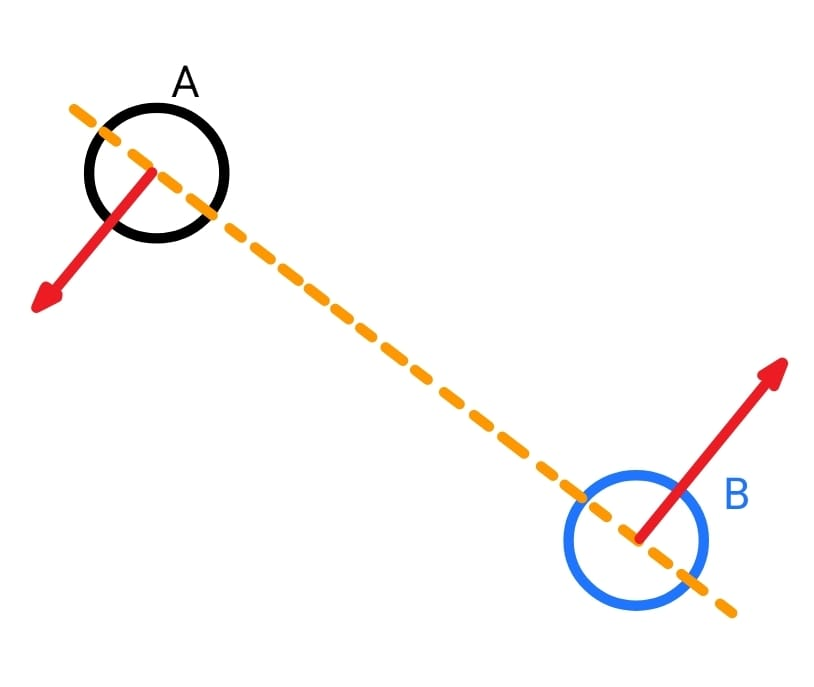
\includegraphics[width=4.5cm]{weakthirdlaw.jpeg}
			\caption{Situación del enunciado débil}
			\label{fig: Nthirdweak}
		\end{figure}
	\end{marginfigure}

	\begin{definition}[\textbf{Tercera Ley de Newton o Ley de Acción-Reacción}]
		Considere dos cuerpos denotados como A y B que presentan algún tipo de interacción entre sí, se dice que:
		Toda \textbf{acción} que realice el cuerpo A sobre el cuerpo B le corresponde una \textbf{reacción} que proveniente del cuerpo B. Estas \textbf{acciones} y \textbf{reacciones} corresponden a fuerzas internas del sistema (cuerpos A y B) debido a su interacción, dichas fuerzas poseen la misma magnitud y su dirección es contraria.
		
		\begin{equation}
			\vec{F}_{AB} = - \vec{F}_{BA}
			\label{eq: NThirdlaw}
		\end{equation}

		Para trabajar con esta ley hay que tomar cuenta cierta ambiguedad que nos lleva a los siguientes enunciados de la tercera ley:
		\begin{itemize}
			\item \textbf{Enunciado Fuerte: } Los vectores correspondientes a las fuerzas de \textbf{acción} y \textbf{reacción} se encuentran sobre una misma recta, es decir, sí se conocen las direcciones de las fuerzas de \textbf{acción} y \textbf{reacción} es posible trazar una recta (conocida como línea de acción) que una los vectores de fuerzas y sea paralela a estos. Ver \Figref{fig: Nthirdstrong}
			\item \textbf{Enunciado Débil: } No ocurre lo anterior. Es imposible unir los vectores de las fuerzas de \textbf{acción} y \textbf{reacción} por medio de una recta que sea paralela a ambos vectores. Ver \Figref{fig: Nthirdweak}
		\end{itemize}

		Además de lo anterior, es preciso destacar que la \textbf{Tercera Ley de Newton} \textcolor{red}{no es una ley general de la naturaleza} y se puede establecer que toda fuerza que dependa de velocidades no obedecerá esta ley.
	\end{definition}

	\subsection{Trabajo y Energía}

	\begin{definition}[\textbf{Trabajo}] Corresponde a la cantidad generada al tomar el producto punto de la fuerza ejercida sobre un cuerpo a lo largo de todo su desplazamiento desplazamiento desde una punto A a un punto B.
		\begin{equation}
			W = \int_{A}^{B} \vec{F} \cdot d\vec{r}
			\label{eq: work}
		\end{equation}
	\end{definition}

	\begin{definition}[\textbf{Fuerza conservativa}] Una fuerza $\vec{F}$ es conservativa si se puede escribir de la forma:
		\begin{equation}
			\vec{F} = - \vec{\nabla}V
			\label{eq: conservativeforce}
		\end{equation}
	\end{definition}

	A partir de las Ecuaciones \rref{eq: NSecondlaw} y \rref{eq: work}:

	\begin{align*}
		W & = \int_{A}^{B} \vec{F} \cdot d\vec{r} \; = \; \int_{A}^{B}  \frac{d \vec{p}}{dt} \cdot d\vec{r}
	\end{align*}

	Ejerciendo el producto punto y trabajando por índices:
	\begin{align*}
		W & = \int_{A}^{B} \sum_{i=1}^{3} \frac{d p_{i}}{dt}dr_{i}
	\end{align*}

	Suponiendo que la masa es constante, la derivada temporal del momentum lineal es de la forma: $\frac{d p_{i}}{dt} = m \frac{d v_{i}}{dt}$:

	\begin{align*}
		W & =  \sum_{i=1}^{3} m \int_{A}^{B} \frac{d v_{i}}{dt}dr_{i} =  \sum_{i=1}^{3} m \int_{A}^{B} \frac{d v_{i}}{dt}dr_{i} \frac{dt}{dt}\\ 
		& = \sum_{i=1}^{3} m \int_{A}^{B} d v_{i} \underbrace{\frac{d r_{i}}{dt}}_{= \: v_{i}} \cancelto{1}{\frac{dt}{dt}}\\
		& = \sum_{i=1}^{3} m \int_{A}^{B}  v_{i} d v_{i} =  \sum_{i=1}^{3} m \int_{A}^{B} \frac{1}{2} d \left(v_{i}^{2}\right)\\
		& = \left . \sum_{i=1}^{3} \frac{1}{2} m v_{i}^{2} \right|_{A} ^{B} = \sum_{i=1}^{3} \frac{1}{2} m v_{iB}^{2} - \sum_{i=1}^{3} \frac{1}{2} m v_{iA}^{2}
	\end{align*}

	\begin{definition}[\textbf{Energía Cinética Traslacional}] Corresponde al trabajo necesario para comenzar a mover un cuerpo desde el reposo hasta la rapidez $v$.

		\begin{equation} 
			T =  \frac{1}{2} m \sum_{i=1}^{3} v_{i}^{2}
			\label{eq: Ttras}
		\end{equation}
	\end{definition}

	\begin{theorem}[\textbf{Trabajo - Energía Cinética}]

		\begin{equation}
			W = \Delta T
			\label{eq: workT}
		\end{equation}
		
	\end{theorem}

	Regresando a la definición \Eqref{eq: work} pero ahora tomando la fuerza que es ejercida sobre el cuerpo como una fuerza conservativa, \Eqref{eq: conservativeforce}.

	\begin{align*}
		W &= \int_{A}^{B} \vec{F} \cdot d\vec{r} =  \int_{A}^{B} - \vec{\nabla}V \cdot d\vec{r} = -V_{B} + V_{A}
	\end{align*}

	\begin{definition}[\textbf{Energía Potencial}] Corresponde a la capacidad de un cuerpo de ejercer trabajo se denomina energía potencial. Ahora se presentan algunos ejemplos de energías potenciales.

		\begin{equation}
			V = \left \{ \begin{matrix}
				mgh\\ 
				\\
				\frac{1}{2}kx^{2} \\
				\\
				\frac{-GMm}{r}\\ 
				\\
				\frac{-Kq_{1}q_{2}}{r}\\ 
				\vdots 
				\end{matrix} \right .
		\end{equation}
		
	\end{definition}

	\begin{theorem}[\textbf{Trabajo - Energía Potencial}]

		\begin{equation}
			W = - \Delta V
			\label{eq: workV}
		\end{equation}
		
	\end{theorem}

	\begin{definition}[\textbf{Energía de un sistema}]
		Ante la suposición de que el sistema a tratar tienen masa constante y es un sistema conservativo, la energía total es de la forma:
		\begin{equation}
			E = T + V
			\label{eq: Energy}
		\end{equation}
		
	\end{definition}

	\subsection{Análogo rotacional de las leyes de Newton}

	Ahora se presentarán algunos conceptos importantes y ecuaciones para una descripción sencilla de la mecánica de partículas en rotación. 	
	\begin{marginfigure}
		\begin{figure}[H]
			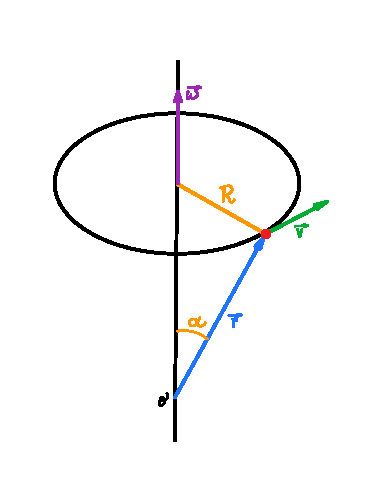
\includegraphics[width=4.8cm]{vwxr.pdf}
			\caption{Relación entre $\vec{v}$ , $\vec{\omega}$ y $\vec{r}$}
			\label{fig: vwxr}
		\end{figure}
	\end{marginfigure}
	Nuevamente se comenzará por los conceptos básicos análogos a los usados en las leyes de Newton y posteriormente se darán las leyes análogas.



	Primero deduciendo una relación entre la velocidad lineal $\vec{v}$ y la velocidad angular $\vec{\omega}$:

	$\bullet$ Se sabe que la velocidad angular es por definición
	\begin{equation}
		\vec{\omega}= \frac{d \vec{\theta}}{dt}
	\end{equation}
	respecto a un eje instantáneo de rotación. Siempre será posible establecer una velocidad angular para un cuerpo en movimiento arbitrário, ya que en cada instante el cuerpo se mueve con una trayectoría circular respecto a un eje de rotación; esto se puede observar en la \Figref{fig: vwxr}.


	Obsevando la rotación infinitesimal presente en \Figref{fig: difvwxr}, se puede concluir la siguiente relación \mn{Recuerde que antes se era bien conocida la relación $v = \omega R$ para una partícula en un movimiento circular de radio $R$ en un plano.\\ 
	\\
	En este caso, al relacionar con $\vec{r}$, se tiene: 
	\begin{center}
		$v = wr sen\left(\alpha\right)$
	\end{center}}
	

	\begin{equation*}
		\delta \vec{r} = \delta \vec{\theta} \times \vec{r}
	\end{equation*}

	Dividiente entre $\delta t$:

	\begin{equation*}
		\frac{\delta \vec{r}}{\delta t} =\frac{\delta \vec{\theta}}{\delta t}  \times \vec{r}
	\end{equation*}

	Lo cual, al considerar $\delta t \rightarrow 0$, se convierte en:

	\begin{equation*}
		\frac{d \vec{r}}{dt} = \frac{d \vec{\theta}}{dt} \times \vec{r}
	\end{equation*}

	\begin{definition}[\textbf{Relación velocida Lineal - Angular}]
		Para un cuerpo en un movimiento arbitrário se cumple lo siguiente para cada instante del movimiento.
		\begin{equation}
			\vec{v} = \vec{w} \times \vec{r}
			\label{eq: vwrelation}
		\end{equation}
		Recuerde que el eje de rotación instantáneo puede cambiar si el movimiento no es una rotación fija.
	\end{definition}


	\begin{marginfigure}
		\begin{figure}[H]
			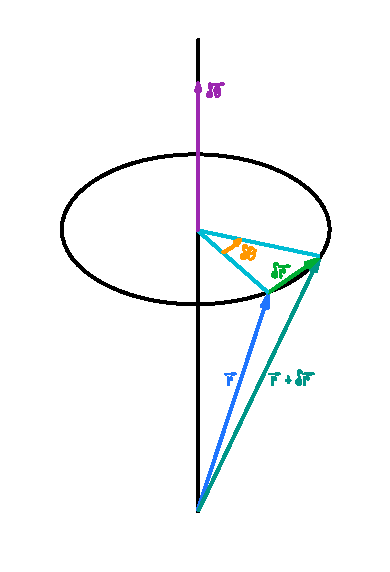
\includegraphics[width=5cm]{difvwxr.pdf}
			\caption{Relación diferencial entre $\vec{v}$ , $\vec{\omega}$ y $\vec{r}$}
			\label{fig: difvwxr}
		\end{figure}
	\end{marginfigure}

	\begin{definition}[\textbf{Torque}]
		El torque es el análogo de la fuerza para las rotaciones. Por lo que el torque corresponde a una interacción del sistema con su entorno que es capaz de generar un cambio en el estado \textit{rotacional} del sistema, dicha interacción es mediada por la presencia de una o más fuerzas y se define como:
		\begin{equation}
			\vec{N}_{\mathcal{O}} = \vec{r} \times \vec{F}
			\label{eq: torque}
		\end{equation}
		Como tal, el torque depende del origen que se este utilizando, debido a su dependencia con el vector posición $\vec{r}$. Al torque es común llamarlo en algunos campos como: torca, momento de fuerza o simplemente momento.
	\end{definition}

	\begin{definition}[\textbf{Momentum Angular}]
		Corresponde al análogo angular del momentum lineal. Es una cantidad vectorial que para el caso de partículas se define como:
		\begin{equation}
			\vec{L}_{\mathcal{O}} = \vec{r} \times \vec{p} = m\; \vec{r} \times \vec{v} = m\; \vec{r} \times \left(\vec{\omega} \times \vec{r} \right) \textup{\textcolor{blue}{\mn{$\vec{A} \times \left(\vec{B} \times \vec{C}\right) = \vec{B} \left(\vec{A}\cdot\vec{B}\right) - \vec{C}\left(\vec{A} \cdot \vec{B}\right)$}}} = m \left[\vec{r}\;^{2} \vec{\omega} - \vec{r} \left(\vec{r} \cdot \vec{\omega}\right)\right]
			\label{eq: momentumA}
		\end{equation}

		De forma similar al torque, el momentum angular depende del origen desde el que se decida medir.\\

		En la amplia gama de casos en que se trabaja con partículas, se podrá reconocer que el producto $\vec{r} \cdot \vec{\omega} = 0$ y los vectores $\vec{r}$ y $\vec{\omega}$ apuntan en una única dirección, por lo que el momentum angular tomará la siguiente forma:

		\begin{equation}
			L_{\mathcal{O}q} = m  r^{2} \omega_{q}
		\end{equation}
	\end{definition}

	\marginnote{La \textbf{masa} \textit{inercial} y los \textbf{ momentos de inercia}  están intimamente relacionados, ambos son medidas de que tan difícil es mover un cuerpo de cierta forma.}

	\begin{definition}[\textbf{Momentos de Inercia}]
		La inercia es el análogo rotacional de la masa y corresponde a una medida que indica que tan difícil es girar un cuerpo respecto a cada eje (A mayor inercia más complicado es girar el objeto). Girando un cuerpo es posible concluir que se pueden generar rotaciones respecto a 3 ejes y por lo tanto \textbf{existen 3 momentos de inercia}, los cuales no necesariamente serán iguales, esto dependerá de la distribución de la masa respecto a cada eje.

		En el caso de partículas puntuales, la inercia se define como:
		
		\begin{equation}
			I_{q}^{\mathcal{O}} = \sum_{i} m_{i} r^{2}_{i}
			\label{eq: easyinercia}
		\end{equation}

		Donde $r_{i}$ corresponde a la distancia que hay entre el eje de rotación y la masa puntual.

	\end{definition}

	\marginnote{El termino \textit{inercial} es para hacer una distinción entre la \textbf{masa inercial} (La masa dada por la aceleración de un cuerpo al estar bajo el efecto de una fuerza) y la \textbf{masa gravitacional} (La masa determinada por las fuerzas gravitacionales entre el cuerpo de interés y otros cuerpos), a pesar de que ambas cantidades \textbf{son iguales} por el princiopio de equivalencia. }

	\begin{definition}[\textbf{Primera Ley de Newton análoga rotacional}]
		De forma similar a la Primera Ley de Newton, este princiopio análogo estable que un cuerpo en un estado rotacional de equilibrio tenderá a mantener dicho estado hasta que un torque neto diferente de cero lo perturbe.
		\begin{equation}
			\sum \vec{N}_{\mathcal{O}} = 0
			\label{eq: Nfirstlawrot}
		\end{equation}
		
	\end{definition}

	\begin{definition}[\textbf{Segunda Ley de Newton análoga rotacional}]
		\begin{equation}
			\sum \vec{N}_{\mathcal{O}} = \frac{d \vec{L}_{\mathcal{O}}}{dt} = \dot{\vec{L}}_{\mathcal{O}}
			\label{eq: NSecondlawrot}
		\end{equation}

		Manteniendo la inercia constante, la ecuación se escribe de la forma:
		\begin{equation}
			\sum N_{q} = I_{q} \alpha_{q}
		\end{equation}
		Donde el subíndice denota el eje respecto al cual se está realizando la suma de torques.
	\end{definition}

	\newpage
	\begin{definition}[\textbf{Tercera Ley de Newton análoga rotacional}] 
		Este principio se enuncia de forma análoga a la Tercera Ley de Newton original bajo la salvedad de que en vez de trabajar con fuerzas, este trabaja con torques.

		\begin{equation}
			\vec{N}_{AB} = - \vec{N}_{BA}
			\label{eq: NThirdlawrot}
		\end{equation}
		
	\end{definition}

	\begin{definition}[\textbf{Energía Cinética Rotacional}]
		Corresponde al trabajo necesario para hacer rotar un cuerpo desde el reposo hasta la rapidez angular $\omega$.
		\begin{equation}
			T_{rot} = \frac{1}{2}I_{q}\omega^{2}
			\label{eq: Trot}
		\end{equation}
		La forma de obtener esta expresión es similar al procedimiento que se realizó con la energía cinética traslacional.
	\end{definition}

	\subsection{Teoremas de Conservación}

	A continuación se van a enunciar los teoremas de conservación bajo la suposición de masa constante y que el sistema a tratar no posee fuerzas disipativas.


	\begin{theorem}[\textbf{Conservación de la Energía}]
		Una vez ya conocida la expresión para la energía del sistema \Eqref{eq: Energy}, basta con derivarla con respecto al tiempo para determinar que restricciones se plantean para la conservación de dicha cantidad:

		\begin{align*}
			E = T + V \Rightarrow \frac{dE}{dt} & = \frac{dT}{dt} + \frac{dV}{dt} \; \textup{; A partir de \Eqref{eq: Ttras} y suponiendo $V = V(\vec{r}, t)$}\\
												& = \frac{d}{dt} \left(\frac{1}{2} m \dot{\vec{r}}\:^{2}\right) + \overbrace{\sum_{i=1}^{3} \frac{\partial V}{\partial x_{i}} \frac{d x_{i}}{d t}}^{= \vec{\nabla}V \cdot \dot{\vec{r}}} + \cancelto{0}{\frac{\partial V}{\partial t}} \; \; ; \left .\begin{matrix}
													\textup{Sistema}\\ 
													\textup{conservativo}
													\end{matrix} \right . \Rightarrow V = V(\vec{r}) \\
												& = \frac{1}{2} m \left(\ddot{\vec{r}} \cdot \dot{\vec{r}} + \dot{\vec{r}} \cdot \ddot{\vec{r}}\right) + \vec{\nabla} V \dot{\vec{r}} 
												= m \ddot{\vec{r}} \cdot \dot{\vec{r}} + \vec{\nabla} V \dot{\vec{r}}
												= \left[m \ddot{\vec{r}} +   \vec{\nabla} V \right] \dot{\vec{r}}\\
												& = \left[\vec{F} + \vec{\nabla} V \right] \cdot \dot{\vec{r}}\\
		\end{align*}

		Para que la energía se conserve se cumple:

		\begin{align*}
			\Rightarrow \frac{dE}{dt} = \left[\vec{F} + \vec{\nabla} V \right] \cdot \dot{\vec{r}} = 0
			&\Rightarrow \vec{F} + \vec{\nabla} V = 0\\
			& \Rightarrow \vec{F} = - \vec{\nabla} V 
		\end{align*}

		\begin{equation}
			\therefore \frac{dE}{dt} = 0 \Rightarrow  \vec{F} = - \vec{\nabla} V
			\label{eq: Econs}
		\end{equation}
		
	\end{theorem}

	\begin{theorem}[\textbf{Conservación de Momentum Lineal}]
		Conociendo ya la expresión de la \Eqref{eq: momentuml}, se derivará con respecto al tiempo para determinar las condiciones en que se conserva dicha cantidad:

		\begin{align*}
			\vec{p} = m \dot{\vec{r}} \Rightarrow \frac{d\vec{p}}{dt} &= \cancelto{0}{\frac{dm}{dt}} \dot{\vec{r}} + m \ddot{\vec{r}}\\ 
																	& = m \ddot{\vec{r}} = \vec{F}
		\end{align*}

		Para que el momentum lineal se conserve se cumple: 

		\begin{align*}
			\Rightarrow \frac{d\vec{p}}{dt} = m \ddot{\vec{r}} = \vec{F} = \vec{0}
		\end{align*}


		\begin{equation}
			\therefore \frac{d\vec{p}}{dt} = 0 \Rightarrow \vec{F} = \vec{0}
			\label{eq: momentumlcons}
		\end{equation}
		
	\end{theorem}

	\begin{theorem}[\textbf{Conservación de Momentum de Angular}]
		A partir de la expresión de la \Eqref{eq: momentumA} y derivandola respecto al tiempo:
		\begin{align*}
			\vec{L}_{\mathcal{O}} = \vec{r} \times \vec{p} \Rightarrow \frac{d \vec{L}_{\mathcal{O}}}{dt} & = \overbrace{\dot{\vec{r}} \times \vec{p}}^{\dot{\vec{r}} \: \parallel \: \vec{p} } + \vec{r} \times \dot{\vec{p}} \\ 
			& = \vec{r} \times \dot{\vec{p}} \; \; \; \textup{; Por la \Eqref{eq: NSecondlaw}} \\ 
			& =  \vec{r} \times \vec{F} \; \; \; \textup{; Por la \Eqref{eq: torque}} \\
			& = \vec{N}_{\mathcal{O}}
		\end{align*}
		Para que se conserve el momentum angular se debe cumplir:

		\begin{equation*}
			\frac{d \vec{L}_{\mathcal{O}}}{dt}= \vec{N}_{\mathcal{O}} = \vec{0}
		\end{equation*}

		\begin{equation}
			\therefore \frac{d \vec{L}_{\mathcal{O}}}{dt} = 0 \Rightarrow  \vec{N}_{\mathcal{O}} = \vec{0}
			\label{eq: momentumAcons}
		\end{equation}
	\end{theorem}



	\subsection{Problemas resueltos}

	\section{Sistemas de partículas}
	\label{sec: sisparticulas}




	\begin{theorem}[\textbf{Teorema de Ejes paralelos}]
		\begin{equation}
			I_{{q}'}= I_{q}^{cm} + Md^{2}
		\end{equation}

		La demostración de este teorema tal y como se encuentra escrito aquí se le dejará al lector y se recomienda verlo como una simplificación del teorema de ejes paralelos real que se desarrollará más adelante.
	\end{theorem}
	
	\section{Sistemas no inerciales}
	\label{sec: noinerciales}


\end{document}